\chapter{Introduction}

The internet has become an integral part of modern life, connecting people all over the world and enabling access to a vast amount of information and resources. It has transformed the way we communicate, do business, and access entertainment. In addition, the internet has made it easier for people to access education, healthcare, and government services, and has helped to bridge the digital divide between those who have access to technology and those who do not.
If an area experiences a loss of connectivity due to natural disasters or lacks access to the internet, the residents of that area will be unable to utilize these services. The COVID-19 pandemic highlighted the importance of internet access as a fundamental necessity and the challenges faced by those who do not have reliable internet connections. According to a report by the United Nations (UN), the pandemic exacerbated existing inequalities and has disproportionately affected people living in rural and underserved areas, who have limited or no access to the internet~\cite{unreport}.

Delay-tolerant networks (DTNs) are a type of networking technology that can be used to deliver internet connectivity to remote areas where traditional networking infrastructure is unavailable or unreliable. DTNs are designed to operate in these environments that cannot rely on continuous connectivity ~\cite{dtn_intro}. They use a store and forward mechanism; a node receiving data from a sender stores the data and waits for a connection to be established with the recipient. When a connection is established, the node forwards the data to the recipient. This process is repeated at each intermediate node along the path until the data reaches its final destination. This allows DTNs to function in scenarios where there is a high degree of network disruption as is the case in remote, disaster-stricken areas and space communications as well.


\section{Project Overview} 

\begin{figure}[ht!]
\centering
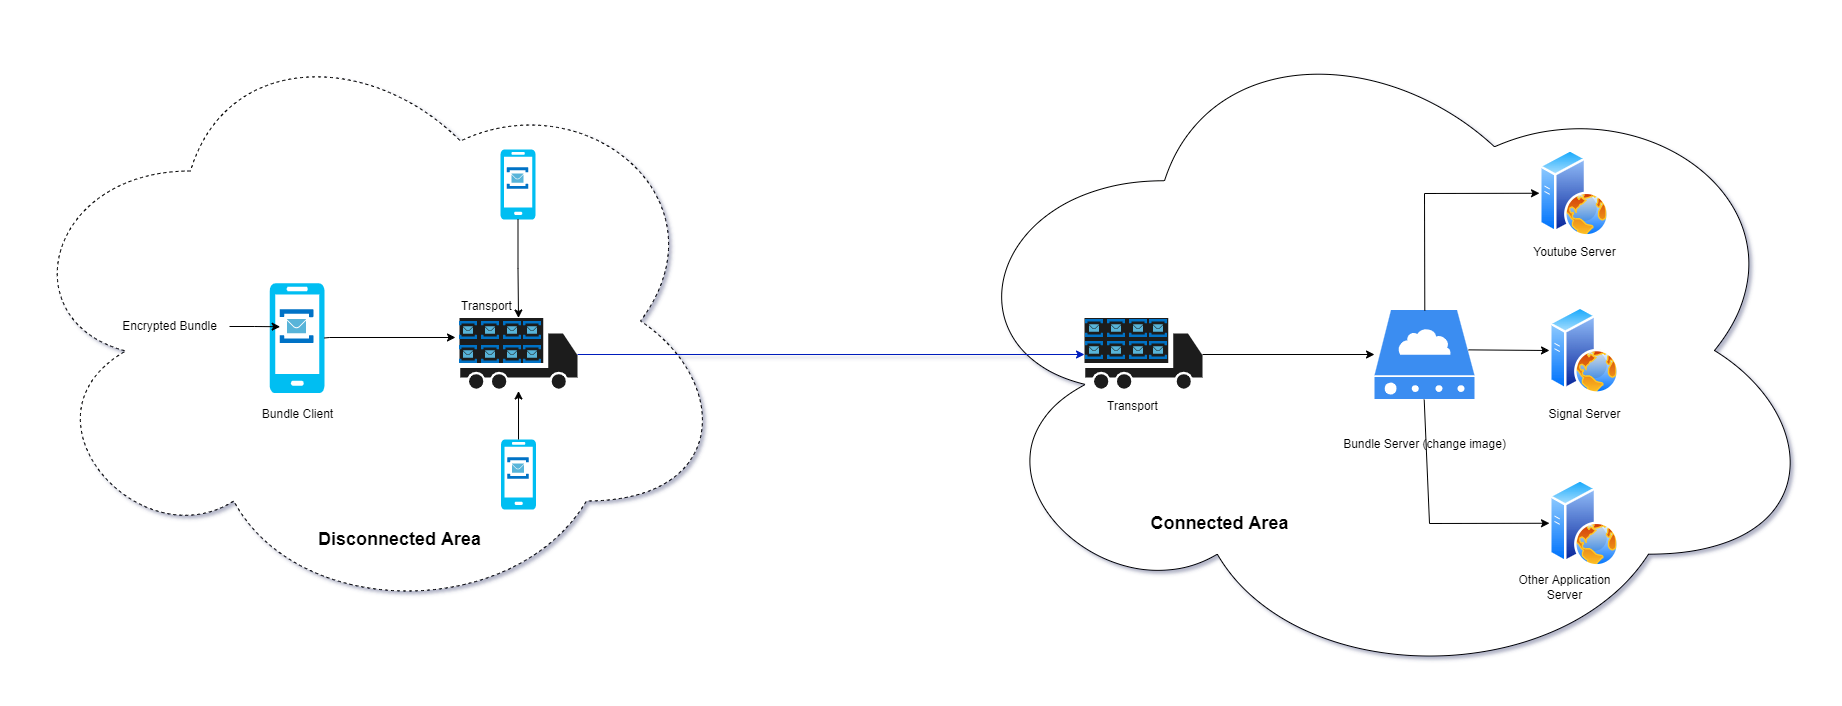
\includegraphics[width= 150mm]{./images/Introduction.png}
\caption{Project Overview}
\end{figure}

To typeset text, you type whatever you want. Multiple spaces are
ignored                           when typesetting, and
the end of a line is treated as another space.
Consequently, when you are typing, you can break lines anywhere, like here
or here,
since the lines are formatted automatically when you typeset the document.
You start a new paragraph by leaving a blank line.

See how easy it is to start a new paragraph? A blank line does the trick.


\section{Special Characters}

Typesetting text is generally pretty easy. However, there are some special
characters that will not be typeset as you might expect. In the remainder of this
section we consider some of the most common of these
special characters. 

The backslash ``\verb+\+'' is used 
as the ``escape'' character, meaning that
whatever follows a backslash is interpreted as a macro.
For example, when \verb+\LaTeX+ is typeset, it looks like \LaTeX, which 
is a lot different from LaTeX.

To get double quotes, use two single quotes. That is, the left double quote is ``, while the right double
quote is ''. When you do it correctly, quoted text looks ``like this.''
If you use the double quote key, you will always get right-quotes, which looks "like this," and is
almost certainly not what you want.

%A tilde ``\verb+~+'' is used as a ``tie,'' that is, a space is inserted, but no line break can occur.
For example, you might type Dr.~Stamp just to be sure that the line of text
does not break between Dr. and Stamp, as it otherwise might.

The percent sign is used for comments---everything following a percent sign 
on a given line is ignored when you \LaTeX\ your file. % Like this stuff here
If you want a percent sign to appear in your document, use \verb+\%+, 
which will give you this \%.

The dollar sign also has special meaning, since it is used to start and end
math formulas. To typeset a dollar sign, use \verb+\$+, like this~\$.

To force \LaTeX\ to insert a space, use a backslash followed by
a space, that is, \verb+\ +. You can put in multiple extra spaces\ \ \ \ \ \ \ if you want.

\section{Fonts}

To change fonts, enclose the text in curly brackets and give the appropriate font command.
For example, to italicize text, {\it do this}, and to get boldface, {\bf this is the ticket}.
Another useful font is {\tt this one}, which produces a typewriter-like font.


\section{Math Basics}

Math typesetting is a big, big, big topic---here we just cover some of
the most basic issues. For more information, look online.

The dollar sign is used to start and end math formulas, like~$\pi r^2$.
If you want your formula displayed on a line by itself, then double
dollar signs
$$
  d(X,Y) =  \sum_{i,j} |x_{ij} - y_{ij}| 
$$
are your friend.

In math formulas, text gets typeset as math symbols. To
insert regular text in a math formula, you can use the \verb+\mbox+
command. Here is an example of a displayed equation with text
$$
  {n\choose 26} 26!\;  26^{n-26} < 26^n \approx 2^{4.7n} \mbox{ is a pretty formula} .
$$ 


\subsection{Numbered Equations}

One of the most useful features of \LaTeX\ is its symbolic cross-references.
What this means is that you can give names to equations, figures, tables, citations, etc., and
refer to those equations, figures, tables, citations, etc., by their names. Then when you \LaTeX\
the document, the correct numbers will magically appear in place of the
names. This is very convenient when you move things around or you insert or delete
stuff. You should definitely use this feature as much as possible.

In this section, we discuss numbered equations, Then in Chapter~\ref{chap:blah}
we consider other examples of symbolic cross-referencing.
Again, this is a feature you should use, since it will save
you a lot of time in the long run.

To typeset a displayed equation with a number, you can 
use \verb+\begin{equation}+ to begin the equation, and \verb+\end{equation}+
to end the equation. You also want to provide a label for the equation.
For example,
\begin{equation}\label{eq:swaps}
  \sum_{i = 1}^{26} m_i \bigg( n - \sum_{j=1}^i m_j \bigg) 
    = n^2 - \sum_{i = 1}^{26} m_i  \sum_{j=1}^i m_j = \sum_{i=1}^{25} \sum_{j=i+1}^{26} m_i m_j 
\end{equation}
gives us a numbered equation. 

Note that labels can be used for
just about anything that is numbered. Generally, to refer to a label,
we use \verb+\ref{label}+, but for equations, you probably want to use
\verb+\eref{label}+, since that will put parenthesis around the number.

So, we can now refer to equation~\eref{eq:swaps} anywhere in the paper.
Better yet, if we move, insert, or delete text, the numbering will still be correct.


\subsection{Last Word on Equations}

Again, typesetting equations is a big topic and we have only given the most basic
of basics here. Just remember that almost anything is possible, and there
are plenty of good resources available. 


\section{Lists}

Numbered lists are not difficult. Here is an example
of a numbered list:
\begin{enumerate}
\item Let $\mbox{\tt score} = \infty$
\item Construct an initial {\tt putativeKey} 
\item Parse the ciphertext using {\tt putativeKey}
\item Compute {\tt newScore} based on the resulting putative plaintext
\item If $\mbox{\tt newScore} < \mbox{\tt score}$ then 
let $\mbox{\tt key} = \mbox{\tt putativeKey}$ and $\mbox{\tt score} = \mbox{\tt newScore}$
\item Modify {\tt key} to obtain a new {\tt putativeKey}
\item Goto~3
\end{enumerate}

Bulleted lists are similar to numbered lists. Here is an example of a bulleted list:
\begin{itemize}
\item How can we determine an initial putative key?
\item  How can we systematically modify the key?
\item Given a putative key, how can we compute a score?
\end{itemize}


\section{Verbatim}

To force \LaTeX\ to typeset exactly what you type, you might want to use the \verb+\verb+
macro. Here is an example:
\verb+four score    and seven+. Note that everything between the ``+'' signs
is typeset as it appears. 

If you happen to have a lot of verbatim text, you can use the verbatim environment,
like this:

\begin{verbatim}
Four score
and seven
years
ago.........
\end{verbatim}

Generally, verbatim should be used sparingly, if at all. But, since
verbatim text has already appeared several times in this document, I thought it
should be explained.

